\begin{name}
{Sở GD Hà Nam}
{ĐỀ THI THỬ TỐT NGHIỆP THPT--NĂM 2022 }
\end{name}
\Opensolutionfile{ans}[hanam]
\begin{ex} %{Cau 1}
Tập nghiệm của bất phương trinh $3^{x}<2$ lả.
\choice
{$\left(-\infty ; \log _{2} 3\right)$}
{\True $\left(-\infty ; \log _{3} 2\right)$}
{$\left(\log _{2} 3 ;+\infty\right)$}
{$\left(\log _{3} 2 ;+\infty\right)$}
\end{ex}

\begin{ex} %{Cau 2}
Cho khối chóp có diện tích đáy $B$ và chiều cao $h$. Thế tich $V$ của khối chóp đã cho được tính theo công thức nào dưới đây?
\choice
{$V=B h$}
{$V=\frac{4}{3} B h$}
{\True $V=\frac{1}{3} B h$}
{$V=\frac{1}{6} B h$}
\end{ex}

\begin{ex} %{Cau 3}
Cho số phức $z$ thỏa mãn $(2+i) z=4-3 i$. Phần ảo của số phức $\bar{z}$ bằng 
\choice
{\True $2$}
{$-3$}
{$-2$}
{$3$}
\end{ex}

\begin{ex}%{Cau 4}
Tiệm cận đứng của đồ thị hàm số $y=\frac{x-1}{x+2}$ là đường thẳng có phương trình
\choice
{$x=1$}
{$y=1$}
{\True $x=-2$}
{$x=2$}
\end{ex}

\begin{ex}%{Cau 5}
Cho hình nón có bán kinhh đáy $r$ và độ dài đường sinh $l$. Diện tích xung quanh $S_{x q}$ của hình nón đã cho được tính theo công thức nào dưới đây?
\choice
{$S_{x q}=\frac{4}{3} \pi r l$}
{$S_{x q}=2 \pi r l$}
{$S_{x q}=4 \pi r l$}
{\True $S_{x q}=\pi r l$}
\end{ex}

\begin{ex}%{Cau 6}
\immini[thm]{Hàm số nào dưới đây có đồ thị là đường cong trong hình bên?
\choice[1]
{$y=x^{3}-3 x-2$}
{\True$y=x^{3}-3 x+2 $}
{$y=x^{4}-2 x^{2}+2$}
{$y=-x^{3}+3 x+2$}
}
{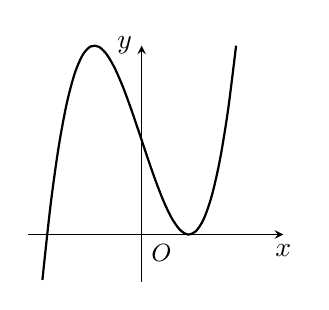
\begin{tikzpicture}[scale=.6]
\draw[-stealth] (-2.4,0) -- (3,0) node[below]{$x$};
\draw[-stealth] (0,-1) -- (0,4) node[left]{$y$};
\draw (0,0) node[below right]{\small $O$};
\draw[thick,smooth] plot[domain=-2.1:2](\x,{(\x)^3-3*(\x)+2});
\end{tikzpicture}
}
\end{ex}

\begin{ex} %{Cau 7}
Cho hàm số $y=f(x)$ có bảng biến thiên như sau:
\\ \centerline{

\begin{tikzpicture}
\tkzTabInit[nocadre,lgt=1.2,espcl=2.2]
{$x$ /.6,$f'(x)$ /.6,$f(x)$ /1.5}
{$-\infty$,$-4$,$0$,$4$,$+\infty$}
\tkzTabLine{,-,$0$,+,$0$,-,$0$,+,}
\tkzTabVar{+/ $+\infty$ ,-/$-6$,+/$1$,-/$-6$,+/$+\infty$}
\end{tikzpicture}
}\\
Hàm số đã cho nghịch biến trên khoảng nào dưới đây?
\choice
{$(-6 ; 1)$}
{\True $(0 ; 3)$}
{$(1 ;+\infty)$}
{$(-\infty ;-2)$}
\end{ex}

\begin{ex} %{Cau 8}
Môđun của số phức $z=-1+3 i$ bằng
\choice
{10}
{$\sqrt{2}$}
{\True $\sqrt{10}$}
{2}
\end{ex}

\begin{ex} %{Cau 9}
Thể tích $V$ của khối nón có bán kinh đáy $r$, chiều cao $ h$ được tinh theo công thức nảo đưới đây?
\choice
{\True $V=\frac{1}{3} \pi r^{2} h$}
{$V=\frac{4}{3} \pi r^{2} h$}
{$V=\pi r^{2} h$}
{$V=\frac{2}{3} \pi r^{2} h$}
\end{ex}

\begin{ex} %{Cau 10}
Với$a>0$, biểu thức $\log _{3}(a \sqrt{3})$ bằng
\choice
{\True $\frac{1}{2}+\log _{3} a$}
{$\frac{1}{2} \log _{3} a$}
{$\sqrt{3} \log _{3} a$}
{$\log _{3} a-\frac{1}{2}$}
\end{ex}

\begin{ex} %{Cau 11}
Cho hình lập phương $A B C D \cdot A^{\prime} B^{\prime} C^{\prime} D^{\prime}$. Góc giừa hai đường thẳng $A^{\prime} B$ và $C D$ bằng
\choice
{$30^{\circ}$}
{\True $45^{\circ}$}
{$90^{\circ}$}
{$60^{\circ}$}
\end{ex}

\begin{ex} %{Cau 12}
Trong không gian $Oxyz$, cho hai điểm $A(2 ;-5 ;-3)$ và $B(1 ; 3 ;-1)$. Mặt phằng đi qua $A$ và vuông góc với đường thẳng $A B$ có phương trình là
\choice
{$-x+8 y+2 z-32=0$}
{$-2 x+5 y+3 z+21=0 $}
{\True $-x+8 y+2 z+48=0$}
{$-x+8 y-2 z+16=0$}
\end{ex}

\begin{ex} %{Cau 13}
Trong không gian $Oxyz$, tọa độ tâm của mặt cầu $(S):(x-2)^{2}+(y+1)^{2}+z^{2}=9$ là
\choice
{\True $(2 ;-1 ; 0)$}
{$(1 ; 1 ; 1)$}
{$(2 ;-1 ; 3)$}
{$(-1 ; 2 ; 0)$}
\end{ex}

\begin{ex} %{Cau 14}
Cho các số thực đương $a, b$ thỏa mãn $\log _{3} a+2 \log _{3} b=1$, khằng định nảo dưới đây đúng?
\choice
{$3 a=2 b$}
{\True $a b^{2}=3$}
{$6 a b=1$}
{$a=3 b^{2}$}
\end{ex}

\begin{ex} %{Cau 15}
Cho hàm số $f(x)$ có bảng xét dấu của $f^{\prime}(x)$ như sau
\\ \centerline{

\begin{tikzpicture}
\tkzTabInit[nocadre,lgt=1.2,espcl=2.2]
{$x$ /.6,$f'(x)$ /.6}
{$-\infty$,$-3$,$0$,$2$,$3$,$+\infty$}
\tkzTabLine{,+,$0$,-,$0$,+,$0$,-,$0$,+,}
\end{tikzpicture}
}\\
Số điểm cực trị của hàm số đã cho là
\choice
{$1$}
{$3$}
{\True $4$ }
{$2$}
\end{ex}

\begin{ex} %{Cau 16}
Tiệm cận ngang của đồ thị hàm số $y=\dfrac{2x+3}{x-1} $ là đường thẳng có phương trình
\choice
{\True $y=2$}
{$y=3$}
{$x=1$}
{$y=-3$}
\end{ex}

\begin{ex} %{Cau 17}
Nghiệm của phương trình$ \log_2{x-1}=3$ là
\choice
{$x=7$}
{$x=4$}
{\True$x=9$}
{$x=3$}
\end{ex}

\begin{ex} %{Cau 18}
\immini[thm]{Cho hàm số $y=a x^3+b x^2+c x+d\quad (a, b, c, d \in \mathbb{R})$ có đồ thị là đường
 cong trong hình bên. Giá trị cực tiểu của hàm số đã cho bằng
\choice
{$0$}
{$1$}
{$3$}
{\True $-1$}
}{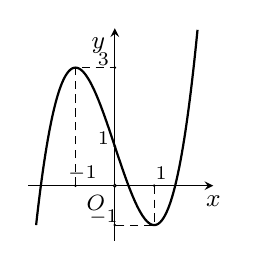
\begin{tikzpicture}[scale=.5]
\draw[-stealth] (-2.2,0) -- (2.5,0) node[below]{\small $x$};
\draw[-stealth] (0,-1.4) -- (0,4) node[below left]{\small $y$};
\draw [thin,densely dashed] (-1,0)|-(0,3) (1,0)|-(0,-1);
\draw[thick,smooth,samples=100] plot[domain=-2:2.1](\x,{(\x)^3-3*(\x)+1});
\draw [fill=white,draw=black] (0,0) circle (1pt)node[below left]{\footnotesize $O$};
\foreach \x in{-1,1}\draw(\x,0) circle (.5pt) node[shift={(60:5pt)}]{\scriptsize $\x$};
\foreach \y in{-1,1,3}\draw(0,\y) circle (.5pt) node[shift={(145:5pt)}]{\scriptsize $\y$};
\end{tikzpicture}}
\end{ex}

\begin{ex} %{Cau 19}
Cho số phức $z=-2+3 i$, khi đó $3 z$ bằng 
\choice
{$-6+3i$}
{\True $-6+9i$}
{$6-9i$}
{$-2+9i$}
\end{ex}

\begin{ex} %{Cau 20}
Nếu $\int_{-2}^{3} f(x) \mathrm{d} x=-2$  thì $\int_{-2}^{3} 3 f(x) \mathrm{d} x$ bằng 
\choice
{$3$}
{\True$-6$}
{$1$}
{$-5$}
\end{ex}

\begin{ex} %{Cau 21}
Trong các hàm số đưới đây, hàm số nào không có cực trị ?
\choice
{$y=-3 x^{3}+2 x$}
{$y=3 x^{3}-2 x$}
{$y=2 x^{3}-x$}
{\True$y=-2 x^{3}-3 x$}
\end{ex}

\begin{ex} %{Cau 22}
Trên khoảng $(0 ;+\infty)$ họ nguyên hàm của hàm số $f(x)=\sqrt[3]{x}$ là
\choice
{$\int f(x) ~\mathrm{d} x=3 x^{\frac{1}{3}}+C$}
{$\int f(x) ~\mathrm{d} x=\frac{1}{3} x^{\frac{1}{3}}+C$}
{$\int f(x) ~\mathrm{d} x=\frac{1}{4} x^{\frac{4}{3}}+C$}
{\True$\int f(x) ~\mathrm{d} x=\frac{3}{4} x^{\frac{4}{3}}+C$}
\end{ex}

\begin{ex} %{Cau 23}
Giao điểm của đồ thị hàm số $y=-3 x^{3}+5 x-2$ với truc tung có tọa độ là
\choice
{$(1 ; 0)$}
{$\left(\frac{2}{3} ; 0\right)$}
{$\left(0 ; \frac{2}{3}\right)$}
{\True $(0 ;-2)$}
\end{ex}

\begin{ex} %{Cau 24}
Cho hàm số $f(x)=2 x-3 \sin x$. Khẳng định nào dưới đây đúng ?
\choice
{$\int f(x) ~\mathrm{d} x=x^{2}-3 \cos x+ C $}
{\True $\int f(x) ~\mathrm{d} x=x^{2}+3 \cos x+ C $}
{$\int f(x) ~\mathrm{d} x=2-3 \cos x+ C $}
{$\int f(x) ~\mathrm{d} x=2+3 \cos x+ C $}
\end{ex}

\begin{ex} %{Cau 25}
Cho khối lăng tru có điện tích đáy bẳng $5$ và chiều cao bằng$ 3$ . Thể tích của khối lãng trụ đã cho bằng
\choice
{$24$}
{$45$}
{\True $15$}
{$5$}
\end{ex}
\begin{ex} %{Cau 26}
Trến mặt phẳng tọa độ, cho $M(-3 ; 1)$ là điểm biều diễn của số phức $z$. Phần thực của $z$ bằng
\choice
{\True$-3$}
{$1$}
{$3$}
{$-1$}
\end{ex}
\begin{ex} %{Cau 27}
Trong không gian $O x y z$, cho hai vectơ $\vec{a}=(-1 ; 3 ;-3)$ và $\vec{b}=(2 ; 1 ;-2)$. Tọa độ của vecto $\vec{b}-\vec{a}$ là
\choice
{\True $(3 ;-2 ; 1)$}
{$(1 ; 4 ;-5)$}
{$(1 ;-2 ; 3)$}
{$(3 ; 2 ;-1)$}
\end{ex}
\begin{ex} %{Cau 28}
Điểm nào dưói đây \textbf{không} thuộc đồ thị hảm số $y=x^{4}-x^{2}-5$ ?
\choice
{$(1;-5)$}
{$(-1;-5)$}
{\True$(-2;6)$}
{$(2;7)$}
\end{ex}
\begin{ex} %{Cau 29}
Trong không gian $O x y z$,  đường thẳng $ d: \frac{x+1}{2}=\frac{y-2}{-1}=\frac{z}{3}$  đi qua điêm nào dưới đây?
\choice
{$A(2 ;-1 ; 3)$}
{\True $C(-1 ; 2 ; 0)$}
{$B(0 ; 2 ;-1)$}
{$D(1 ;-2 ; 0)$}
\end{ex}
\begin{ex} %{Cau 30}
Nếu $\int_{1}^{2} f(x) ~\mathrm{d} x=3$ và $\int^{2} g(x) ~\mathrm{d} x=-2$ thì $\int^{2}[f(x)-g(x)] ~\mathrm{d} x$ bằng
\choice
{$1$}
{\True $5$}
{$-5$}
{$6$}
\end{ex}
\begin{ex} %{Cau 31}
Trong không gian $Oxyz$, mặt phẳng $(P):x-4 y+5 z-2=0$ có một vectơ pháp tuyến là:
\choice
{$\overrightarrow{u_{1}}=(-1 ; 4 ; 5)$}
{\True $\overrightarrow{u_{2}}=(1 ;- 4 ; 5)$}
{$\overrightarrow{u_{3}}=(5 ; -4 ; 1)$}
{$\overrightarrow{u_{4}}=(-4 ; 5 ; -2)$}
\end{ex}
\begin{ex} %{Cau 32}
Trên đoạn $\left[\frac{1}{3} ; \frac{3}{2}\right]$, hàm số $y=2 x^{2}+\frac{1}{2 x}$ đạt giá trị nhỏ nhất tại điểm
\choice
{$x=\frac{1}{2}$}
{\True$x=\frac{3}{2}$}
{$x=1$}
{$x=\frac{1}{3}$}
\end{ex}
\begin{ex} %{Cau 33}
Tập xác định của hàm số $y=x^{\sqrt{5}}$ là
\choice
{\True$(0 ;+\infty)$}
{$\mathbb{R}$}
{$\mathbb{R} \backslash\{0\}$}
{$(5 ;+\infty)$}
\end{ex}
\begin{ex} %{Cau 34}
Trên khoảng $(0 ;+\infty)$, đạo hàm của hàm số $y=\log _{\sqrt{3}} x$ là
\choice
{$y^{\prime}=\frac{1}{2 x \ln \sqrt{3}}$}
{$y^{\prime}=\frac{\sqrt{3}}{x \ln 3}$}
{$y^{\prime}=\frac{\sqrt[3]{3}}{x}$}
{\True$y^{\prime}=\frac{1}{x \ln \sqrt{3}}$}
\end{ex}
\begin{ex} %{Cau 35}
Nếu $\int_{-1}^{2} f(x) \mathrm{d} x=3$ thì $\int_{-1}^{2}[f(x)-4 x] \mathrm{d} x$ bằng
\choice
{$1 $}
{$4$}
{$-5$}
{\True $-3$}
\end{ex}
\begin{ex} %{Cau 36}
Gọi $z_{1}, z_{2}$ là các nghiệm phức của phương trình $z^{2}-2 z+17=0$. Giá trị của biểu thức $3\left(z_{1}+z_{2}\right)-z_{1} z_{2}$ bằng 
\choice
{\True $-11$}
{$23$}
{$16$}
{$-8$}
\end{ex}
\begin{ex} %{Cau 37}
Cho hinh nón đỉnh $S$, đường tròn đáy có tâm $O$ và góc ở đỉnh bẳng $120^{\circ}$. Một mặt phẳng đi qua $S$ cắt hình nón theo thiết diện là tam giác vuông $S A B$. Biết khoảng cách giữa hai đường thẳng $A B$ và $S O$ bằng 3 , diện tích xung quanh của hinh nón đã cho bằng
\choice
{$12 \pi \sqrt{3}$}
{$27 \pi \sqrt{3}$}
{\True $18 \pi \sqrt{3}$}
{$9 \pi \sqrt{3}$}
\end{ex}

\begin{ex} %{Cau 38}
Số giao điểm của đồ thị hàm số $y=x^3+4x^2-11x-30$ với trục hoành là 
\choice 
{ $0$}
{ $1$}
{ $2$}
{\True $3$} 
\end{ex} 
\begin{ex} %{Cau 39}
Trong không gian $Oxyz$, cho điểm $A( 3;\,1;\,-2 )$. Đường thẳng đi qua $A$ và song song với đường thẳng\\ $\Delta:\dfrac{x}{2}=\dfrac{y+1}{-1}=\dfrac{z-2}{1}$ có phương trình là
\choice 
{\True $\heva{
& x=3+2t \\ 
& y=1-t \\ 
& z=-2+t \\ 
}$}
{ $\heva{
& x=2+3t \\ 
& y=-1+t \\ 
& z=1-2t \\ 
}$}
{ $\heva{
& x=-3+2t \\ 
& y=-1-t \\ 
& z=2+t \\ 
}$}
{ $\heva{
& x=3-2\,t \\ 
& y=1+t \\ 
& z=-2+t \\ 
}$} 
\end{ex} 

\begin{ex} %{Cau 40}
Trong không gian $Oxyz$, cho điểm $A( 1;1;2 )$ và hai đường thẳng ${{d}_{1}}:\heva{
& x=3+t \\ 
& y=-1+2t \\ 
& z=4 \\ 
}$ và ${{d}_{2}}:\dfrac{x+2}{1}=\dfrac{y}{1}=\dfrac{z-2}{2}$. Đường thẳng qua $A$, cắt đường thẳng ${{d}_{1}},{{d}_{2}}$ có phương trình là
\choice 
{ $\dfrac{x-1}{1}=\dfrac{y-1}{1}=\dfrac{z-2}{-1}$}
{ $\dfrac{x-1}{1}=\dfrac{y-1}{-1}=\dfrac{z-2}{1}$} 
{\True $\dfrac{x-1}{2}=\dfrac{y-1}{1}=\dfrac{z-2}{1}$}
{ $\dfrac{x-1}{1}=\dfrac{y-1}{2}=\dfrac{z-2}{-1}$} 
\end{ex} 
\begin{ex} %{Cau 41}
Trên tập hợp các số phức, cho phương trình ${{z}^2}+az+b=0,\,\,( a,\,b\in \mathbb{R} )$. Biết phương trình đã cho có hai nghiệm là ${{z}_{1}}=2-i$ và ${{z}_{2}}$, khi đó giá trị của $\bigg| a{{z}_{1}}-b{{z}_{2}} \bigg|$ bằng 
\choice 
{ $6\sqrt{10}$}
{ $18$}
{ $15\sqrt{3}$}
{\True $5\sqrt{13}$} 
\end{ex} 
\begin{ex} %{Cau 42}
Cho hai hàm số $f( x )=ax^3+bx^2+cx-4$ và $g( x )=dx^2+ex+2,\ ( a,\ b,\ c,\ d,\ e\in \mathbb{R} )$. Biết rằng đồ thị hàm số $y=f( x )$ và $y=g( x )$ cắt nhau tại $3$ điểm có hoành độ lần lượt là $-3;\ -1;\ 2$. Hình phẳng giới hạn bởi đồ thị hai hàm số đã cho có diện tích bằng.
\choice 
{ $\dfrac{316}{15}$}
{ $\dfrac{191}{9}$}
{ \True $\dfrac{253}{12}$}
{ $\dfrac{97}{6}$} 
\end{ex}
\Closesolutionfile{ans}